\chapter{Models for \Ttwo relaxation enhancement}\label{ch:models}

As discussed in Chapter \ref{ch:background}, researchers have developed a number of models to explain the decrease in \Ttwo of the water protons in blood.
Thulborn originally applied the Luz-Meiboom equation to describe the decrease in \Ttwo and its dependence on the CPMG echo time\cite{ThulbornOxygenationdependencetransverse1982}.
This assumes that the water protons in blood exchange between two sites with different Larmor frequencies, with a rate $\frac{1}{\tau_{ex}}$.
While this provides good agreement with experimental data, it does not provide a good description of the underlying physical system - for example, the exchange time in found in previous studies do not agree with measurements of the exchange rate across the red blood cell membrane \cite{MeyerNMRrelaxationrates1995}.
There are also inconsistencies in the values of $\tau_{ex}$ reported in the literature, with values ranging from 0.3 ms to 10.1 ms (see table 1 TODO).
Another model has been proposed by Jensen and Chandra, which more describes the dephasing of water protons that diffuse through areas of magnetic field inhomogeneities\cite{JensenNMRrelaxationtissues2000}.
Generally, the two models predict the same behaviour at short echo times (\textless 3 ms) and at long echo times (\textgreater 20ms)\cite{BrooksT2shorteningweaklymagnetized2001}, but in the intemediate range, the two models give different values for the magnitude of the \Ttwo change.
Additionally, experiments comparing the two models have found that at clinical MRI fields (1.5 T and up), both models provide good agreement with experimental data \cite{StefanovicHumanwholebloodrelaxometry2004,GardenerDependencebloodR22010,GrgacHematocritoxygenationdependence2013}.
Because of this, the Luz-Meiboom equation is typically used when analysing data, as it is simpler than the diffusion model.

It is also possible that both mechanisms are occuring together, in which case, it is useful to know the relative contributions of the two processes.
Based on studies of the spectroscopic line width of red blood cell suspensions, Matwiyoff et al. suggest that diffusion processes dominate at higher fields, while exchange between cytoplasm and plasma is more significant at lower fields (\textless 1.5 Tesla)\cite{Matwiyofflineshapeswater1990}.
As another component of this research, the agreement between these models and data collected at lower fields has been tested to investigate whether the different models are more effective at lower field.

\section{Theory}
Thulborn proposed using the Luz-Meiboom equation to describe the decrease in \Ttwo that occurs in deoxygenated blood in the CPMG experiment.
This equation comes from the study of a chemical exchange process, where protons on an ammonium ion exchange with the solvent\cite{LuzNuclearMagneticResonance1963}.
Protons bound to the ammonium ion have a different chemical shift, which combined with the exchange, makes the refocusing pulses in the CPMG experiment less effective.
Luz and Meiboom show that this process leads to a \Ttwo decrease dependent on the echo time given by \autoref{eq:LMchemEx}\cite{LuzNuclearMagneticResonance1963}, where $p_i$ is the fraction of protons in state $i$, $\delta_i$ is the shift of protons in state $i$, $t_{ec}$ is the echo time, and $\tau_{ex}$ is the average time between exchanges. It also includes the $T_{20}$ to include the $T_2$ when there is no exchange contribution.

\begin{equation}
\label{eq:LMchemEx}
\frac{1}{T_2} = \frac{1}{T_{20}} + \sum_i{p_i\delta_i^2} (1 - \frac{t_{ec}}{2\tau_{ex}} \tanh{\frac{2\tau_{ex}}{t_{ec}}})
\end{equation}

\begin{equation}
\label{eq:LMblood}
\frac{1}{T_2} = \frac{1}{T_{20}} +(P_A)(1 - P_A)\tau_{ex} [(1-sO_2)\alpha\omega_0]^2 (1 - \frac{\tau_{ex}}{t_{ec}} \tanh{\frac{\tau_{ex}}{t_{ec}}})
\end{equation}

This was thought to be a similar situation to red blood cells, where the susceptibility change due to haemoglobin causes a difference in the field in the cytoplasm compared to the plamsa, and protons exchange across the cell membrane.
One version of this interpretation is given by Wright\cite{WrightEstimatingoxygensaturation1991}. In \autoref{eq:LMblood} the summation over the states becomes $P_A$, which is the relative population of protons in cytoplasm and plasma (and therefore the haematocrit, and the frequency difference given by a term dependent on the $sO_2$, the field strength $\omega_0$, and a dimensionless factor $\alpha$ which is dependent on the susceptibility change of deoxyhaemoglobin.

One challenge to applying this model comes from the term $\tau_{ex}$.
In the literature, there are a range of values for the exchange time - see % \autoref{tb:exchTime}TODO...
This is typically attributed to using different ranges of $t_ec$ in the CPMG experiments, which can cause the fitting to become biased.
In addition, many of these do not agree with values for the rate of transmembrane exchange when measured by other NMR methods.
This suggests that the exchange time parameter is not necessarily due to exchange across the cell membrane.

A similar formula has been found by Jensen and Chandra, following a more general derivation of the signal in CPMG experiments from protons diffusing in a weakly inhomogeneous field\cite{JensenNMRrelaxationtissues2000}.
Their model uses the weak field approximation, which requires a correlation function $K(t)$ that describes the variations in the magnetic field as protons diffuse.
By approximating this correlation function with a simple exponential decay, they found that the relaxation rate is given by \autoref{eq:LMsimp}\cite{JensenNMRrelaxationtissues2000}.
This has the same form as the Luz-Meiboom formula, but with the exchange time replaced by a more general ``correlation time'', and the factor $K_0$ representing the variance of the magnetic field.
Because of this, their correlation time is not directly connected to an exchange process, which could explain why the Luz-Meiboom formula agrees with experimental results, but also gives a range of exchange times.
\begin{equation}
\label{eq:LMsimp}
\frac{1}{T_2} = \frac{1}{T_{20}} + \gamma^2 K_0 (1 - \frac{2\tau_{ex}}{t_{ec}} \tanh{\frac{2\tau_{ex}}{t_{ec}}})
\end{equation}

By using a different correlation function which describes the diffusion of water molecules around microscopic field inhomogeneities, Jensen and Chandra also derived another formula for the change in \Ttwo.

\begin{equation}
\label{eq:JC}
\frac{1}{T_2} = \frac{1}{T_{20}}+ G_0 \frac{\gamma^2 r_c^2}{2D} F(\frac{4D \Delta t}{r_c^2})
\end{equation}

\begin{displaymath}
\mbox{where  } F(x) = \frac{1}{\sqrt{\pi}} \int_0^\infty \frac{e^{-y}}{\sqrt{y}} \left[1-\frac{1}{xy} \tanh{xy}\right] \mathrm{d}y
\end{displaymath}
Here, $G_0$ is the mean squared magnitude of field inhomogeneities, $r_c$ is their characteristic length scale (i.e. the size of the red blood cells), and $D$ is the diffusion coefficient of water protons.
In studies comparing the two models, it has been shown that the two models agree well enough with experimental data, but differ slightly in the range

\section{Experimental Setup}
To better map out the dependency of \Ttwo on echo time, a wider range of echo times than the 5 used in the other continuous experiments was required.
In this series of experiments, a new pulse sequence  was written to sequentially measure multiple CPMG experiments using a range of echo times specified by the user.
The pulse sequence supports either using a linear range of echo times, or loading a file with the desired echo times.
A list of 13 times between 0.5 - 20 ms was used, with more closely spaced samples in the region between 1 - 5 ms, as this is where the differences in the predictions of the two models are most visible.
To ease processing, the number of echoes in each CPMG experiment is the same.
This presented a problem with measuring longer echo times, for example, 200 echoes at 20 ms requires an experiment time of 4 seconds.
Overall, the experiment with 13 echo times, and a T\textsubscript{R} of 5 seconds takes 5 minutes.

These experiments were completed during the continuous flow experiments, when the blood was in a deoxygenated state, with measurements done at each field strength.
The oxygenation was logged by optical sensor, and probably didn't vary significantly [but actually did it? should probably check TODO!].
A steady flow rate was maintained using the screw clamp, which meant that the blood did not have the chance to settle and meant that the temperature was relatively stable during the 5 minutes of the experiment ( \mbox{$\pm 4^{\circ}\, \mathrm{C}$}) TODO see how much this actually was!!.

\subsection*{Analysis method}
To compare the two models, a similar approach was used to Stefanovic\cite{StefanovicHumanwholebloodrelaxometry2004} and Gardener\cite{GardenerDependencebloodR22010}.
\Ttwo values were calculated for each echo time using least squares fitting of the phased and integrated echo amplitudes with the function $S=Ae^{(t/T_2)}$.
To remove the effect of the fast decaying signal from the tube surrounding the blood, the first 40 ms of the CPMG decay is ignored in the fitting.
The models were then fit to constrained versions of equations \ref{eq:LMsimp} and \ref{eq:JC}  (where either $\tau_{ex}$ or $r_c$ are held constant).
The results from the constrained fit were then used as initial guesses for an unconstrained least squares fit to the formulae, where all three parameters were allowed to vary.
Finally, the sum of squared residuals was calculated to give a quantitative measure of the model's agreement.

\section{Results}

\subsection{\Ttwo Measurement}
CPMG decays were measured for blood in the contunuous flow setup at each of the field strengths used in those experiments.
To obtain a \Ttwo value for each echo time, the echo intensities were fit to a monoexponential decay.
An example of this is shown in \autoref{fig:dm-CPMGdecay}, the section of the decay used for fitting is also marked.

\begin{figure}[h]
\centering
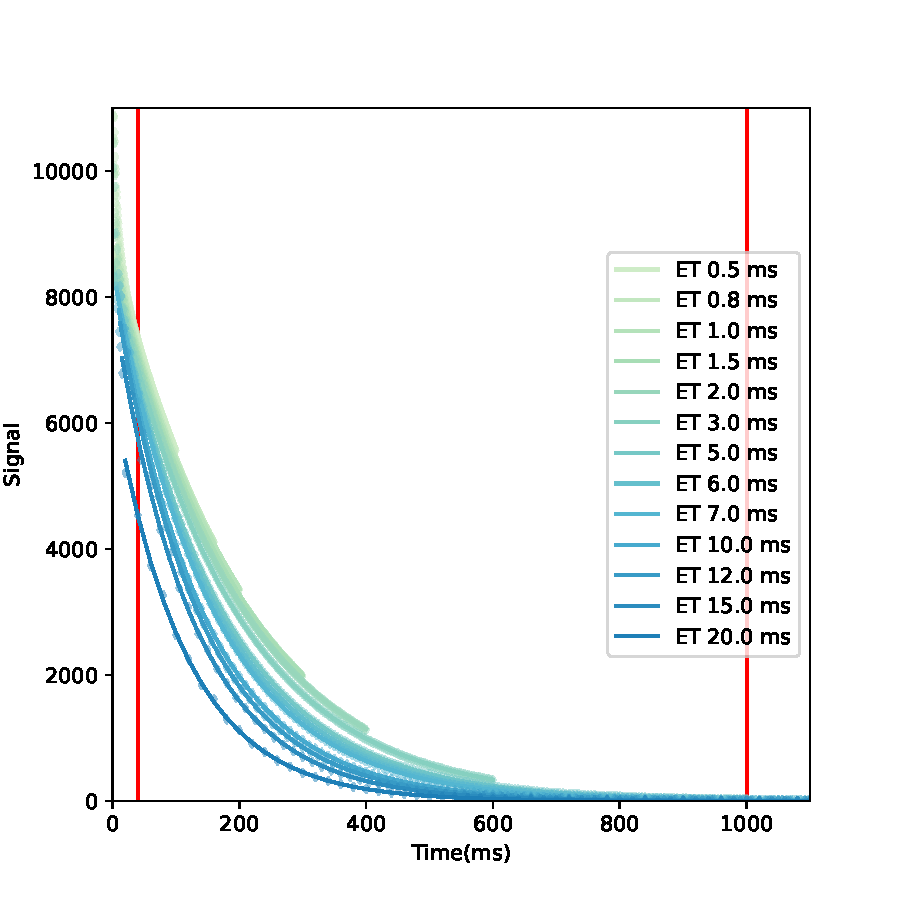
\includegraphics[width=10cm]{figures/diffmodels/20MHzT2fit.pdf}

\caption{CPMG decays measured at the field of 20 MHz, at the different echo times. Red lines indicate data points used for fitting}
\label{fig:dm-CPMGdecay}
\end{figure}

With the exception of the fast decay from the plastic tube at the start of the CPMG experiment, the echo intensities show good agreement with the monoexponential decay function, which confirms that the blood is not separating, and that the decay is not significantly affected by the flow.

Values of \Ttwo measured at each echo time were then used as inputs for fitting equations \ref{eq:LMsimp} and \ref{eq:JC}.
The resulting best fit curves for both equations are shown in \autoref{fig:dm-fitResults}, while the parameters are included in \autoref{tab:dm-fitPars}.


\begin{figure}[t]
  \makebox[\textwidth][c]{

  \begin{subfigure}[t]{0.6\textwidth}
  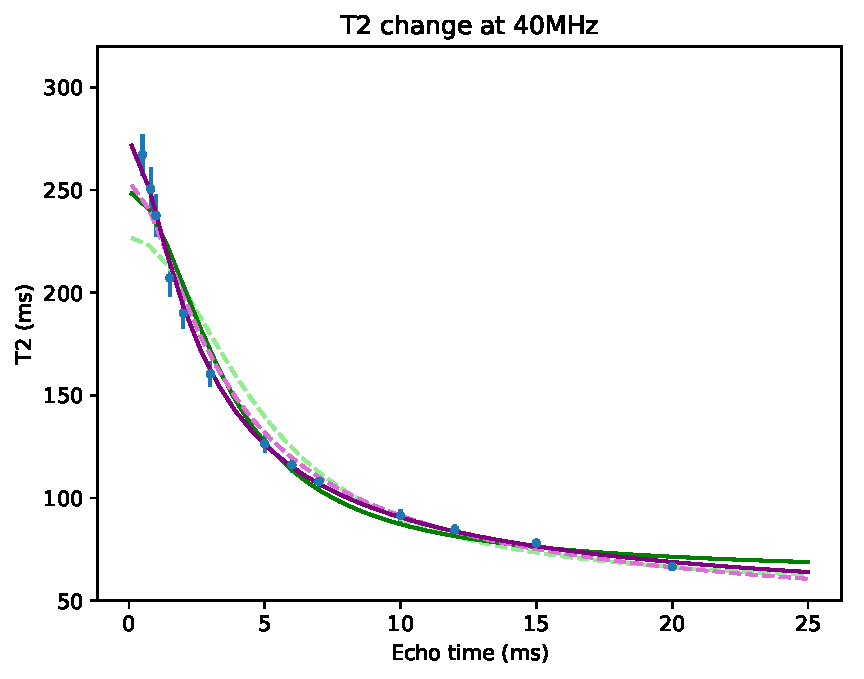
\includegraphics[width=\textwidth]{figures/diffmodels/40MHzT2.pdf}
  \caption{40 MHz}
  \label{fig:dm-fitResults40}
  \end{subfigure}
  \begin{subfigure}[t]{0.6\textwidth}
  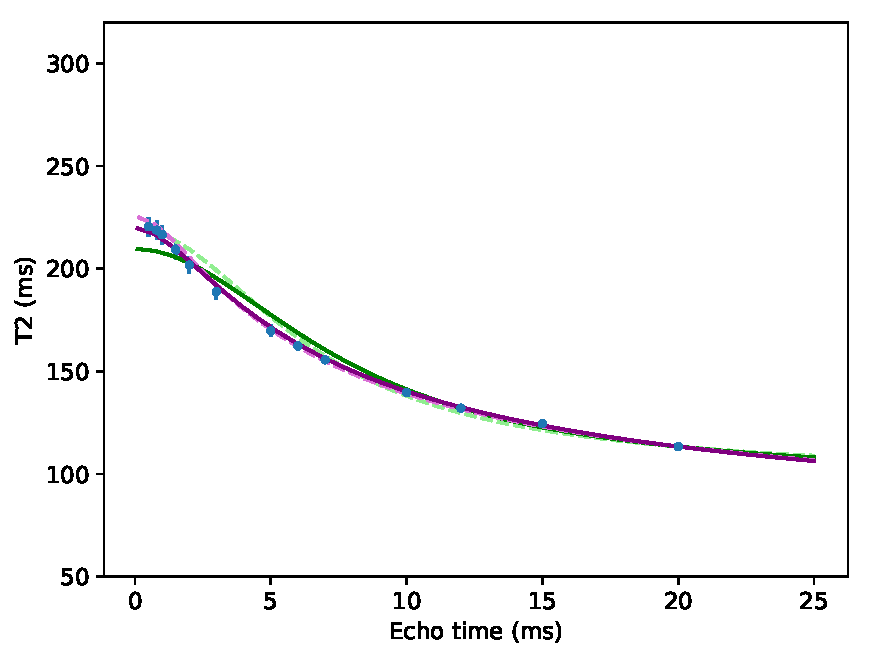
\includegraphics[width=\textwidth]{figures/diffmodels/20MHzT2.pdf}
  \caption{20 MHz}
  \label{fig:dm-fitResults20}
  \end{subfigure}
  \hfill
  }

  \makebox[\textwidth][c]{
  \begin{subfigure}[t]{0.6\textwidth}
  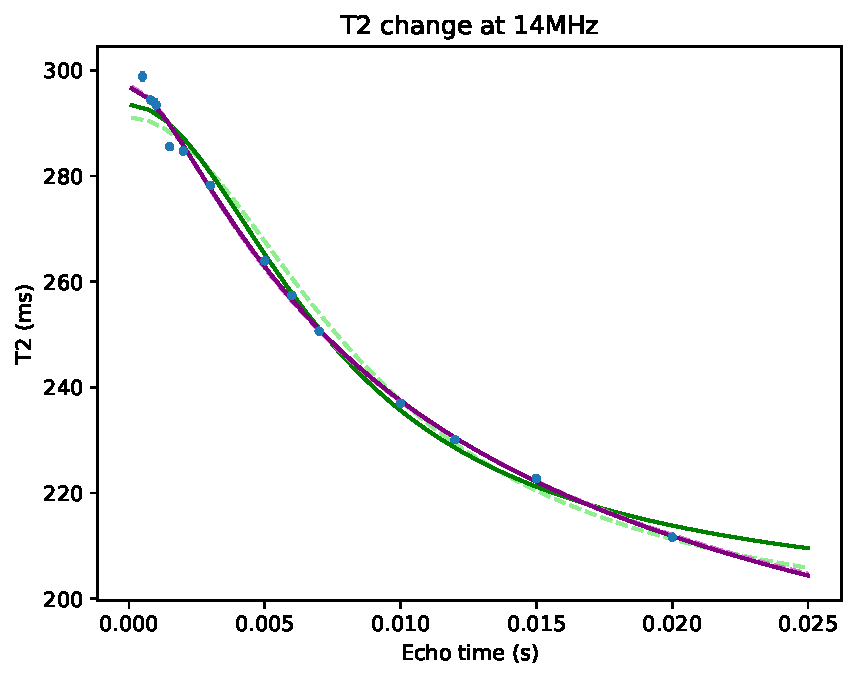
\includegraphics[width=\textwidth]{figures/diffmodels/14MHzT2.pdf}
  \caption{14 MHz}
  \label{fig:dm-fitResults14}
  \end{subfigure}
  \begin{subfigure}[t]{0.6\textwidth}
  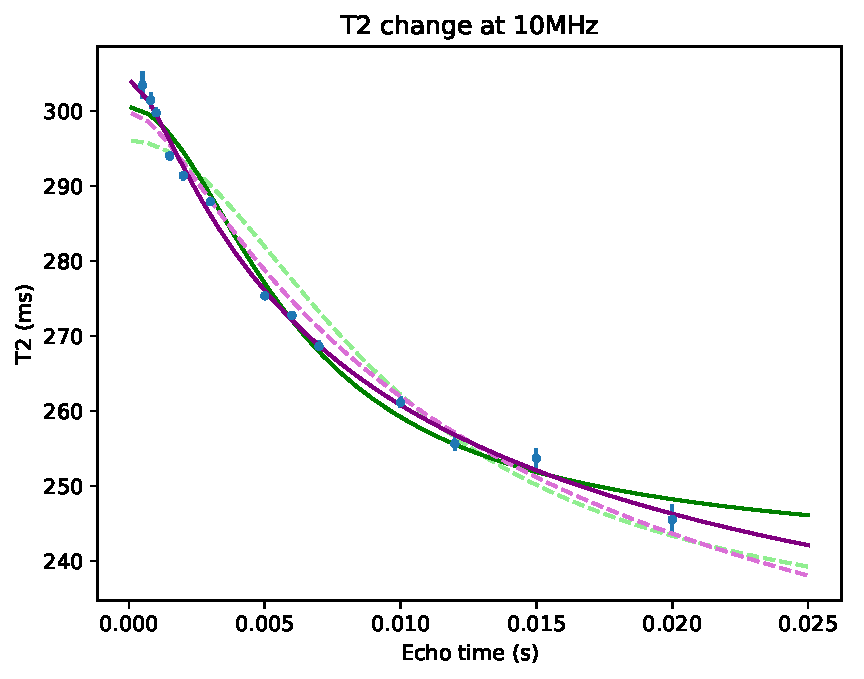
\includegraphics[width=\textwidth]{figures/diffmodels/10MHzT2.pdf}
  \caption{10 MHz}
  \label{fig:dm-fitResults10}
  \end{subfigure}
  \hfill
  }

  \makebox[\textwidth][c]{
  \begin{subfigure}[t]{0.6\textwidth}
  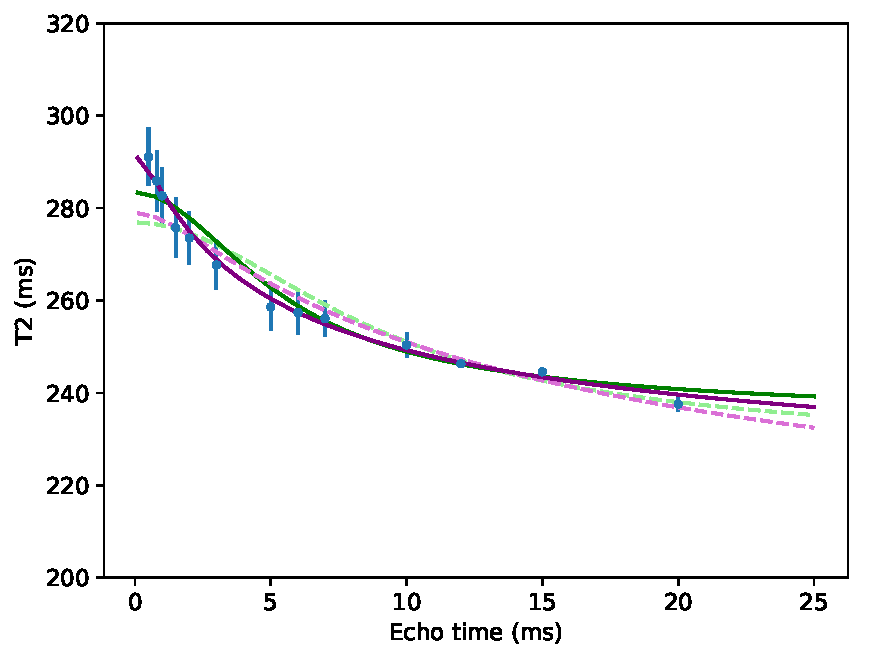
\includegraphics[width=\textwidth]{figures/diffmodels/5MHzT2.pdf}
  \caption{5 MHz}
  \label{fig:dm-fitResults5}
  \end{subfigure}
  \hspace{0.6\textwidth}
  }

  \caption[Luz-Meiboom and diffusion model fits at different fields]{Luz-Meiboom (Green) and diffusion model (Purple) fit to \Ttwo results at different fields. Dashed lines show the best fits when $\tau_{ex}$ is fixed at 3.3 ms and when r\textsubscript{c} is fixed at 4.2 μm. Solid lines show the best fits when all three variables are unconstrained.}
  \label{fig:dm-fitResults}
\end{figure}


\begin{table}
\centering

\makebox[\textwidth][c]{
\begin{tabular}{l|ccc|ccc|}
%Copied from Python/processCPMGvt/newCPMGvt
& \multicolumn{3}{c}{Constrained LM} & \multicolumn{3}{c}{Unconstrained LM} \\ Field
& T\textsubscript{20} & K\textsubscript{0} & Tau\textsubscript{ex}
& T\textsubscript{20} & K\textsubscript{0} & Tau\textsubscript{ex}\\
 & ms & 10\textsuperscript{14} T\textsuperscript{2} & ms & ms & 10\textsuperscript{14} T\textsuperscript{2} & ms \\ \hline
40 MHz & 223 \pm 1.0 & 6.491 \pm 0.026 & 3.30 \cellcolor[gray]{0.9} & 246 \pm 1.5 & 7.646 \pm 0.053 & 2.38 \pm 0.02\\
20 MHz & 209 \pm 0.8 & 2.538 \pm 0.026 & 3.30 \cellcolor[gray]{0.9} & 213 \pm 1.1 & 2.779 \pm 0.046 & 2.71 \pm 0.07\\
14 MHz & 289 \pm 0.1 & 0.821 \pm 0.003 & 3.30 \cellcolor[gray]{0.9} & 292 \pm 0.2 & 0.858 \pm 0.004 & 2.61 \pm 0.03\\
10 MHz & 296 \pm 1.7 & 0.461 \pm 0.026 & 3.30 \cellcolor[gray]{0.9} & 300 \pm 2.3 & 0.612 \pm 0.066 & 2.00 \pm 0.28\\
5M MHz & 284 \pm 0.2 & 0.518 \pm 0.008 & 3.30 \cellcolor[gray]{0.9} & 291 \pm 0.5 & 0.939 \pm 0.029 & 1.02 \pm 0.04\\

%stop copying

\end{tabular}
}

\vspace{1cm}

\makebox[\textwidth][c]{
\begin{tabular}{l|ccc|ccc|}

%Same deal..
& \multicolumn{3}{c}{Constrained JC} & \multicolumn{3}{c}{Unconstrained JC} \\ Field
& T\textsubscript{20} & G\textsubscript{0} & r\textsubscript{c}
& T\textsubscript{20} & G\textsubscript{0} & r\textsubscript{c}\\
 & ms & 10\textsuperscript{14} T\textsuperscript{2} & um & ms & 10\textsuperscript{14} T\textsuperscript{2} & um \\ \hline
40 MHz & 255 \pm 1.4 & 9.657 \pm 0.038 & 4.30 \cellcolor[gray]{0.9} & 272 \pm 2.3 & 10.821 \pm 0.122 & 3.80 \pm 0.04\\
20 MHz & 218 \pm 1.0 & 3.758 \pm 0.038 & 4.30 \cellcolor[gray]{0.9} & 218 \pm 1.4 & 3.757 \pm 0.092 & 4.30 \pm 0.12\\
14 MHz & 297 \pm 0.2 & 1.194 \pm 0.005 & 4.30 \cellcolor[gray]{0.9} & 295 \pm 0.3 & 1.142 \pm 0.008 & 4.65 \pm 0.05\\
10 MHz & 300 \pm 1.9 & 0.689 \pm 0.038 & 4.30 \cellcolor[gray]{0.9} & 304 \pm 3.3 & 0.932 \pm 0.181 & 3.22 \pm 0.50\\
5M MHz & 287 \pm 0.2 & 0.749 \pm 0.011 & 4.30 \cellcolor[gray]{0.9} & 297 \pm 1.0 & 1.674 \pm 0.110 & 2.09 \pm 0.09\\

%Stop thecopy
\end{tabular}
}
\caption{Best fit values to the experimental data at different fields}
\label{tab:dm-fitPars}
\end{table}
At the higher field of 40 MHz (\autoref{fig:dm-fitResults40}), all of the curves show good agreement with the experimental data. The

\section{Discussion}
